\section{Date: 2026-08-21}
\noindent \textbf{Series ID: WFRBST01121} 

\noindent This series is titled Share of Mortgages Held by the Top 1\% (99th to 100th Wealth Percentiles) and has a frequency of Quarterly. The units are Percent of Aggregate and the seasonal adjustment is Not Seasonally Adjusted.The observation start date is 1989-07-01 and the observation end date is 2026-01-01.The popularity of this series is 1. \\ 

\noindent \textbf{Series ID: A900RC1A027NBEA} 

\noindent This series is titled Net government investment: Equipment and software: Consumption of fixed capital (DISCONTINUED) and has a frequency of Annual. The units are Billions of Dollars and the seasonal adjustment is Not Seasonally Adjusted.The observation start date is 1929-01-01 and the observation end date is 2011-01-01.The popularity of this series is 1. \\ 

\subsection{Raw Regression}
\noindent Regresses the two series against each other directly. A significant result here can come just as easily from both series sharing a long-run trend as from any real relationship.

\begin{center}
\begin{tabular}{lclc}
\toprule
\textbf{Dep. Variable:}           & value\_fred\_A900RC1A027NBEA & \textbf{  R-squared:         } &     0.174   \\
\textbf{Model:}                   &             OLS              & \textbf{  Adj. R-squared:    } &     0.133   \\
\textbf{Method:}                  &        Least Squares         & \textbf{  F-statistic:       } &     4.219   \\
\textbf{Date:}                    &       Fri, 21 Aug 2026       & \textbf{  Prob (F-statistic):} &   0.0533    \\
\textbf{Time:}                    &           12:20:58           & \textbf{  Log-Likelihood:    } &   -100.42   \\
\textbf{No. Observations:}        &                22            & \textbf{  AIC:               } &     204.8   \\
\textbf{Df Residuals:}            &                20            & \textbf{  BIC:               } &     207.0   \\
\textbf{Df Model:}                &                 1            & \textbf{                     } &             \\
\textbf{Covariance Type:}         &          nonrobust           & \textbf{                     } &             \\
\bottomrule
\end{tabular}
\begin{tabular}{lcccccc}
                                  & \textbf{coef} & \textbf{std err} & \textbf{t} & \textbf{P$> |$t$|$} & \textbf{[0.025} & \textbf{0.975]}  \\
\midrule
\textbf{const}                    &      50.0857  &       31.671     &     1.581  &         0.129        &      -15.979    &      116.150     \\
\textbf{value\_fred\_WFRBST01121} &       1.8177  &        0.885     &     2.054  &         0.053        &       -0.028    &        3.664     \\
\bottomrule
\end{tabular}
\begin{tabular}{lclc}
\textbf{Omnibus:}       & 11.459 & \textbf{  Durbin-Watson:     } &    0.087  \\
\textbf{Prob(Omnibus):} &  0.003 & \textbf{  Jarque-Bera (JB):  } &    9.487  \\
\textbf{Skew:}          &  1.501 & \textbf{  Prob(JB):          } &  0.00871  \\
\textbf{Kurtosis:}      &  4.158 & \textbf{  Cond. No.          } &     218.  \\
\bottomrule
\end{tabular}
%\caption{OLS Regression Results}
\end{center}

Notes: \newline
 [1] Standard Errors assume that the covariance matrix of the errors is correctly specified.

\begin{figure}
\centering
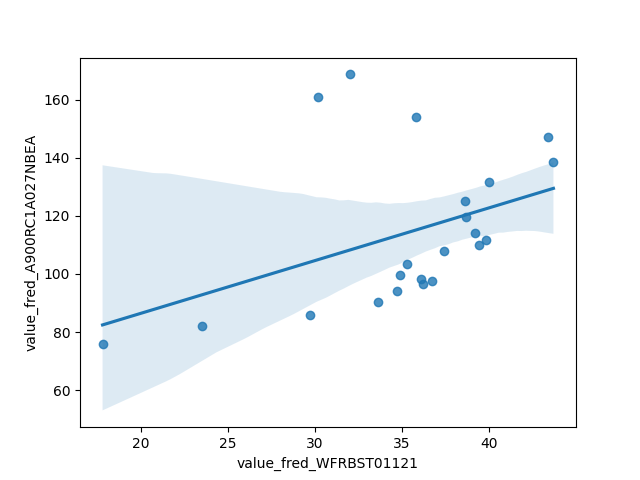
\includegraphics[scale = 0.9]{plots/plot_2026-08-21.png}
\caption{Raw Regression Plot for 2026-08-21}
\end{figure}
\newpage
\subsection{Detrended Regression}
\noindent Regresses the residuals of each series after removing its own linear time trend, so a shared trend can no longer drive the result on its own. A relationship that stays significant here is better evidence of a genuine link between the two series.

\begin{center}
\begin{tabular}{lclc}
\toprule
\textbf{Dep. Variable:}                      & value\_fred\_A900RC1A027NBEA\_detrended & \textbf{  R-squared:         } &     0.333   \\
\textbf{Model:}                              &                   OLS                   & \textbf{  Adj. R-squared:    } &     0.300   \\
\textbf{Method:}                             &              Least Squares              & \textbf{  F-statistic:       } &     9.980   \\
\textbf{Date:}                               &             Fri, 21 Aug 2026            & \textbf{  Prob (F-statistic):} &  0.00494    \\
\textbf{Time:}                               &                 12:20:58                & \textbf{  Log-Likelihood:    } &   -67.369   \\
\textbf{No. Observations:}                   &                      22                 & \textbf{  AIC:               } &     138.7   \\
\textbf{Df Residuals:}                       &                      20                 & \textbf{  BIC:               } &     140.9   \\
\textbf{Df Model:}                           &                       1                 & \textbf{                     } &             \\
\textbf{Covariance Type:}                    &                nonrobust                & \textbf{                     } &             \\
\bottomrule
\end{tabular}
\begin{tabular}{lcccccc}
                                             & \textbf{coef} & \textbf{std err} & \textbf{t} & \textbf{P$> |$t$|$} & \textbf{[0.025} & \textbf{0.975]}  \\
\midrule
\textbf{const}                               &   -1.319e-12  &        1.157     & -1.14e-12  &         1.000        &       -2.412    &        2.412     \\
\textbf{value\_fred\_WFRBST01121\_detrended} &      -0.7473  &        0.237     &    -3.159  &         0.005        &       -1.241    &       -0.254     \\
\bottomrule
\end{tabular}
\begin{tabular}{lclc}
\textbf{Omnibus:}       &  8.387 & \textbf{  Durbin-Watson:     } &    0.366  \\
\textbf{Prob(Omnibus):} &  0.015 & \textbf{  Jarque-Bera (JB):  } &    1.968  \\
\textbf{Skew:}          &  0.039 & \textbf{  Prob(JB):          } &    0.374  \\
\textbf{Kurtosis:}      &  1.537 & \textbf{  Cond. No.          } &     4.89  \\
\bottomrule
\end{tabular}
%\caption{OLS Regression Results}
\end{center}

Notes: \newline
 [1] Standard Errors assume that the covariance matrix of the errors is correctly specified.

\begin{figure}
\centering
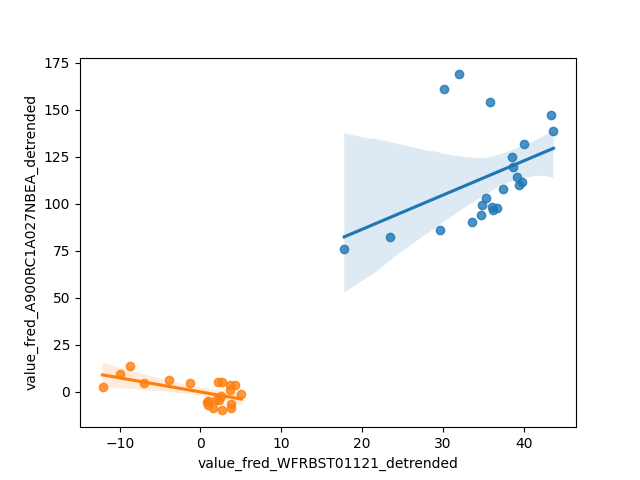
\includegraphics[scale = 0.9]{plots/plot_2026-08-21_detrended.png}
\caption{Detrended Regression Plot for 2026-08-21}
\end{figure}
\newpage
